\documentclass[crop, tikz]{standalone}
\usepackage{tikz}
\usepackage{amsmath}
\usepackage{amssymb}

\usetikzlibrary{positioning, decorations.pathmorphing, shapes}

\begin{document}
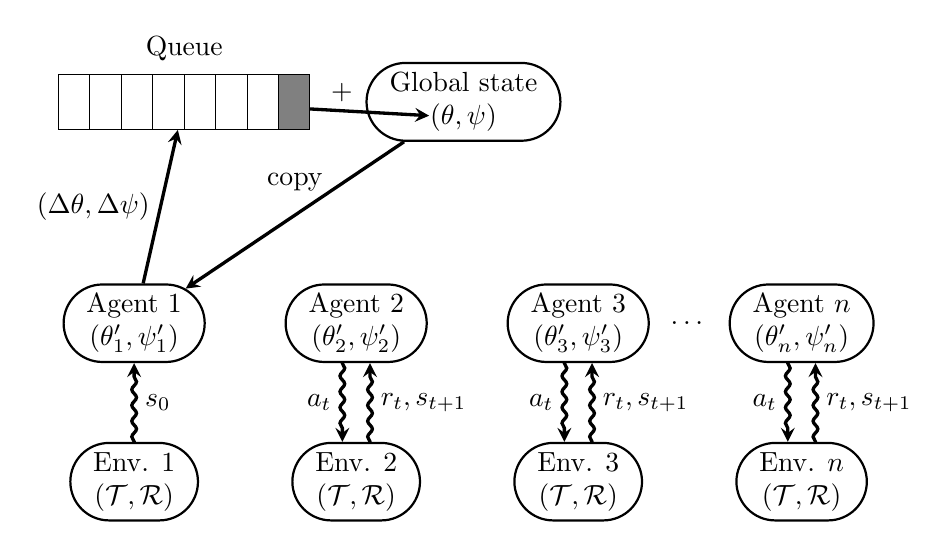
\begin{tikzpicture}	

	\node[rounded rectangle, draw, thick, align=center] (A1) {Agent 1\\$(\theta_1', \psi_1')$};
	\node[rounded rectangle, draw, thick, right= of A1, align=center] (A2) {Agent 2\\$(\theta_2', \psi_2')$};
	\node[rounded rectangle, draw, thick, right= of A2, align=center] (A3) {Agent 3\\$(\theta_3', \psi_3')$};
	\node[right=0.4em of A3, align=center] (mid) {\dots};
		
	\node[rounded rectangle, draw, thick, right= of A3, align=center] (AN) {Agent $n$\\$(\theta_n', \psi_n')$};
		
	\node[rounded rectangle, draw, thick, yshift=8em, xshift=11.9em, align=center] (G) {Global state\\$(\theta, \psi)$};
			
	\node[rounded rectangle, draw, thick, below= of A1, align=center] (E1) {Env. 1\\$(\mathcal{T}, \mathcal{R})$};
	\node[rounded rectangle, draw, thick, below= of A2, align=center] (E2) {Env. 2\\$(\mathcal{T}, \mathcal{R})$};
	\node[rounded rectangle, draw, thick, below= of A3, align=center] (E3) {Env. 3\\$(\mathcal{T}, \mathcal{R})$};
	\node[rounded rectangle, draw, thick, below= of AN, align=center] (EN) {Env. $n$\\$(\mathcal{T}, \mathcal{R})$};
		
	\draw[-stealth, very thick] (G) -- node[above=0.5em] {copy} (A1);
		
	\foreach \x in {2,3,N}
		\draw[-stealth, decoration={snake, pre length=0.01mm, segment length=2mm, amplitude=0.3mm, post length=1.5mm}, decorate,very thick] ([xshift=-0.5em]A\x.south) -- node[left] {$a_t$} ([xshift=-0.5em]E\x.north);
	\foreach \x in {2,3,N}
		\draw[-stealth, decoration={snake, pre length=0.01mm, segment length=2mm, amplitude=0.3mm, post length=1.5mm}, decorate,very thick] ([xshift=0.5em]E\x.north) -- node[right] {$r_t, s_{t+1}$} ([xshift=0.5em]A\x.south);
			
	\draw[-stealth, decoration={snake, pre length=0.01mm, segment length=2mm, amplitude=0.3mm, post length=1.5mm}, decorate,very thick] (E1.north) -- node[right] {$s_0$} (A1.south);
			
	\node[rectangle split,
		minimum height=0.7cm,
		rectangle split horizontal,
		rectangle split parts=8, 
		draw, 
		anchor=center,
		left=2em of G,
		rectangle split part fill={white,white,white,white,white,white,white,gray}] 
		(q1) {};
  
	\node[above=0.1em of q1] (N) {Queue};

	\draw[-stealth, very thick] (A1) -- node[left] {$(\Delta\theta, \Delta\psi)$} (q1);
	\draw[-stealth, very thick] (q1) -- node[above, xshift=-1em] {$+$} ([xshift=2.3em,yshift=-0.5em]G.west);
  
\end{tikzpicture}
\end{document}
